\documentclass[handout]{beamer}
% Januar  2012

%\documentclass{beamer}

%\usetheme{Warsaw}
%\usetheme{Berkeley}
\usetheme{JuanLesPins}
%\usepackage{ngerman}
\usepackage{amsmath}
\usepackage{array}
\usepackage{graphicx}
\usepackage{graphics}
%\usepackage{pgfpages}
\usepackage{psfrag}
\usepackage{chicago}
%\pgfpagelayout{2 on 1}[a4paper,border shrink=5mm]
\newcommand{\tcb}{\color{blue}}
\newcommand{\tcg}{\color{green}}
\newcommand{\tcr}{\color{red}}
\newcommand{\tco}{\color{orange}}
\newcommand{\tcm}{\color{magenta}}
\newcommand{\ftheta}{\mbox{\boldmath $\theta$}}
\newcommand{\btheta}{\mbox{\boldmath $\theta$}}
\newcommand{\feta}{\mbox{\boldmath $\eta$}}
\newcommand{\fnu}{\mbox{\boldmath $\nu$}}
\newcommand{\frho}{\mbox{\boldmath $\rho$}}
\newcommand{\fm}{\mbox{\bf m}}
\newcommand{\m}{\ensuremath{\mathbf m}}
\setbeamertemplate{footline}[page number]
\begin{document}


\title[Le projet Mosaic]
{\bf Le projet Mosaic \\
}
\author[ L. Brummer]{{\bf Ludwig Brummer}\\
\texttt{ludwig.brummer@mytum.de \\
\bf Artem Oboturov}\\
\texttt{oboturov@telecom-paristech.fr} \\
 }
\date{29 janvier 2013}

\begin{frame}
\titlepage
\end{frame}

\begin{frame}
\frametitle{\bf Synoptique} \tableofcontents
\end{frame}



%%%%%%%%%%%%%%%%%%%%%%%%%%%%%%%%%%%%%%%%%%%%%%%%%%%%%%%%%%%%%%%%%%%%%%%%





%%%%%%%%%%%%%%%%%%%%%%%%%%%%%%%%%%%%%%%%%%%%%%%%%%%%%%%%%%%%%%%%%







%%%%%%%%%%%%%%%%%%%%%%%%%%%%%%%%%%%%%%%%%%%%%%%%%%%%%%%%%%%%%%


\section{Organisation de travail sur projet}

\begin{frame}
\begin{center}
{\Huge GitHub}
\end{center}
\begin{figure}[H]

\includegraphics[scale=0.50]{GitHub.png}
\end{figure}
\end{frame}

\begin{frame}
\frametitle{\bf Des probl\`emes...}
\begin{figure}[H]
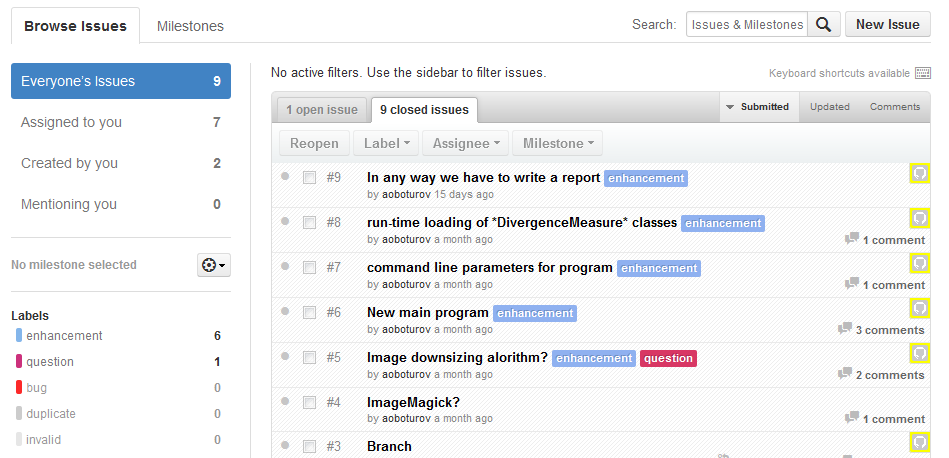
\includegraphics[scale=0.36]{GitHubIssues.png}
\end{figure}
\end{frame}

\begin{frame}
\frametitle{\bf et des solutions}
\begin{figure}[H]
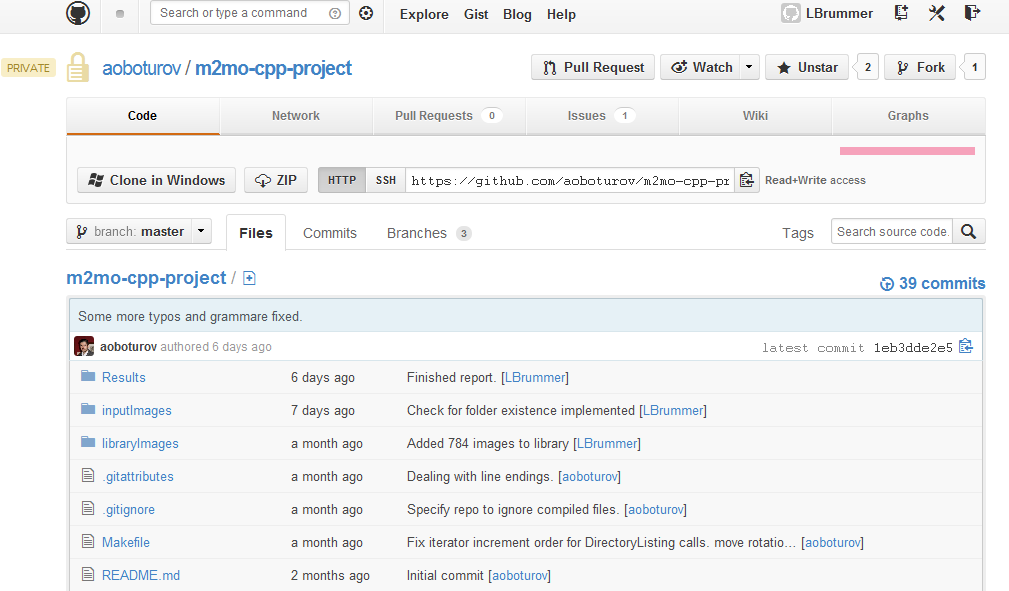
\includegraphics[scale=0.36]{GitHubCommits.png}
\end{figure}
\end{frame}

\section{Instruction d'emploi}
\begin{frame}
\begin{center}
{\Huge Instruction d'emploi}
\end{center}
\end{frame}


\subsection{La biblioth\`eque des carreaux}

\begin{frame}
\frametitle{\bf La biblioth\`eque des carreaux}
Le programme a besoin de quelques images de m\^eme taille pour construire une mosa\"{i}que.
\begin{itemize}
\item {\tcb Location}: Dossier "libraryImages"

\item {\tcb library\_generator}: ex\'ecutable\ avec {-}{-}size ou {-}{-}help

\item {\tcb taille}: {-}{-}size XX
\end{itemize}

\end{frame}

\subsection{Le programme principal}

\begin{frame}
\frametitle{\bf Le programme principal}
Le programme a besoin de quelques images de m\^eme taille pour construire une mosa\"{i}que.
\begin{itemize}
\item {\tcb Location}: Dossier "inputImages"

\item {\tcb options}: ex\'ecutable\ avec {-}{-}tilesize XX, {-}{-}help, {-}{-}mse, {-}{-}meancolor, {-}{-}mcmse

\item {\tcb Resultats}: Dossier "outputImages"
\end{itemize}

\end{frame}

\section{Le logiciel et son code source}

\subsection{Diagramme de classes}

\begin{frame}

\frametitle{\bf Diagramme de classes}
\begin{center}
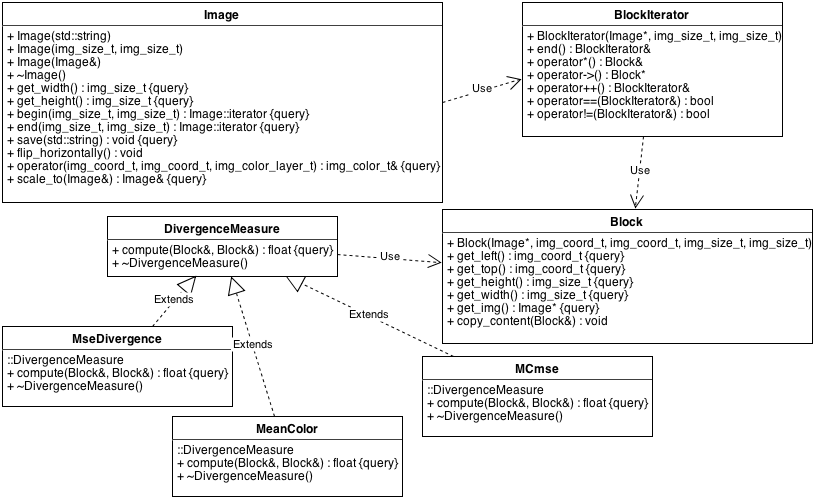
\includegraphics[width=\textwidth]{class_diagram.png}
\end{center}

\end{frame}

\section{Algorithmes}

\subsection{R\'ealisation des algorithmes}
\begin{frame}

\frametitle{\bf Algorithme de cr\'eation de mosa\"ique}
\begin{centering}
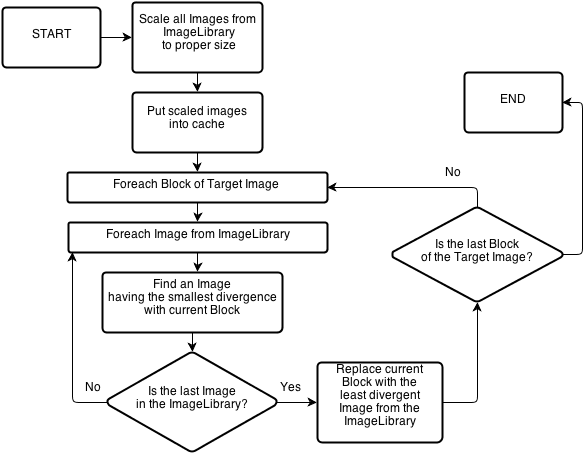
\includegraphics[width=0.75\textwidth]{the_mosaic_creation_algorithm.png}
\end{centering}
\end{frame}

\subsection{L'algorithme de sous\'echantillonnage lin\'eaire}
\begin{frame}
\frametitle{\bf Sous\'echantillonnage}
\begin{figure}[H]
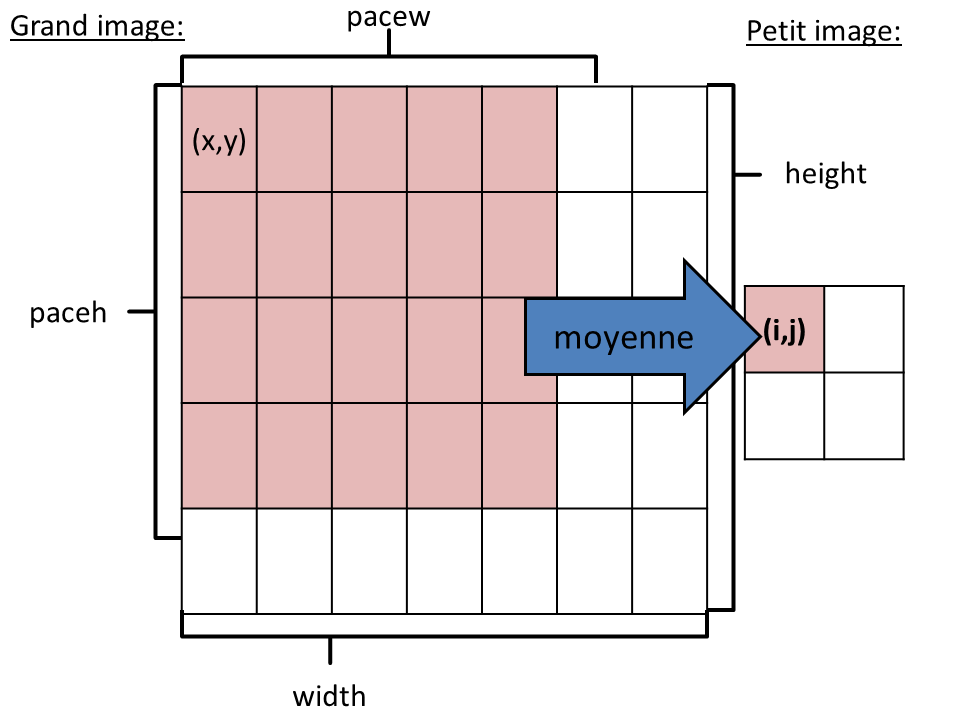
\includegraphics[scale=0.36]{scale_to.png}
\end{figure}
\end{frame}


\subsection{Les mesures de divergence}

\begin{frame}
\frametitle{\bf La mesure d'erreur des moindres carr\'es}
\begin{equation*}
err=\frac{1}{X\cdot Y\cdot C}\sum_{x,y,c}\left(\frac{block(x,y,r,v,b)-tile_{image}(x,y,r,v,b)}{255}\right)^2
\end{equation*}
\end{frame}

\begin{frame}
\frametitle{\bf La mesure de couleurs moyens}
\begin{equation*}
err=\frac{1}{X\cdot Y\cdot C}\sum_{x,y,c}\left|\frac{block(x,y,r,v,b)-tile_{image}(x,y,r,v,b)}{255}\right|
\end{equation*}
\end{frame}
\begin{frame}
\frametitle{\bf La mesure de Monte Carlo}
Soient $(Z_{x,y,c})$ une suite des variables al\'eatoires i.i.d. de la loi Bernoulli avec $p~=~0,25$.
$c\in \{r,v,b\}$ indique le niveau de couleur.
Alors l'erreur est:
\begin{equation*}
err=\frac{1}{\sum_{x,y,c}Z_{x,y,c}}\sum_{x,y,c}\left(\frac{block(x,y,c)-tile_{image}(x,y,c)}{255}\right)^2\cdot Z_{x,y,c}
\end{equation*}
\end{frame}
\section{Resultats}

\begin{frame}
\begin{center}
{\Huge Resultats}
\end{center}
\end{frame}


\begin{frame}
\frametitle{\bf Temps d'\'execution avec des mesures differents}
\begin{table}
\begin{tabular}{|c|c|c|c|}
\hline 
\small Mesure & \small guybrush.jpg & \small IMG\_1293\_small.JPG & \small IMG\_1331.JPG \\ 
\hline 
\small MSE & 1:13 min & 0:38 min & 0:39 min \\ 
\hline 
\small Couleur moyenne & 0:58 min & 0:31 min & 0:29 min \\ 
\hline 
\small Monte Carlo & 0:47 min & 0:25 min & 0:25 min \\ 
\hline 

\end{tabular}
\label{tab:temps}  
\end{table}
\end{frame}

\begin{frame}
\frametitle{\bf Resultat avec MSE }
\begin{figure}[H]
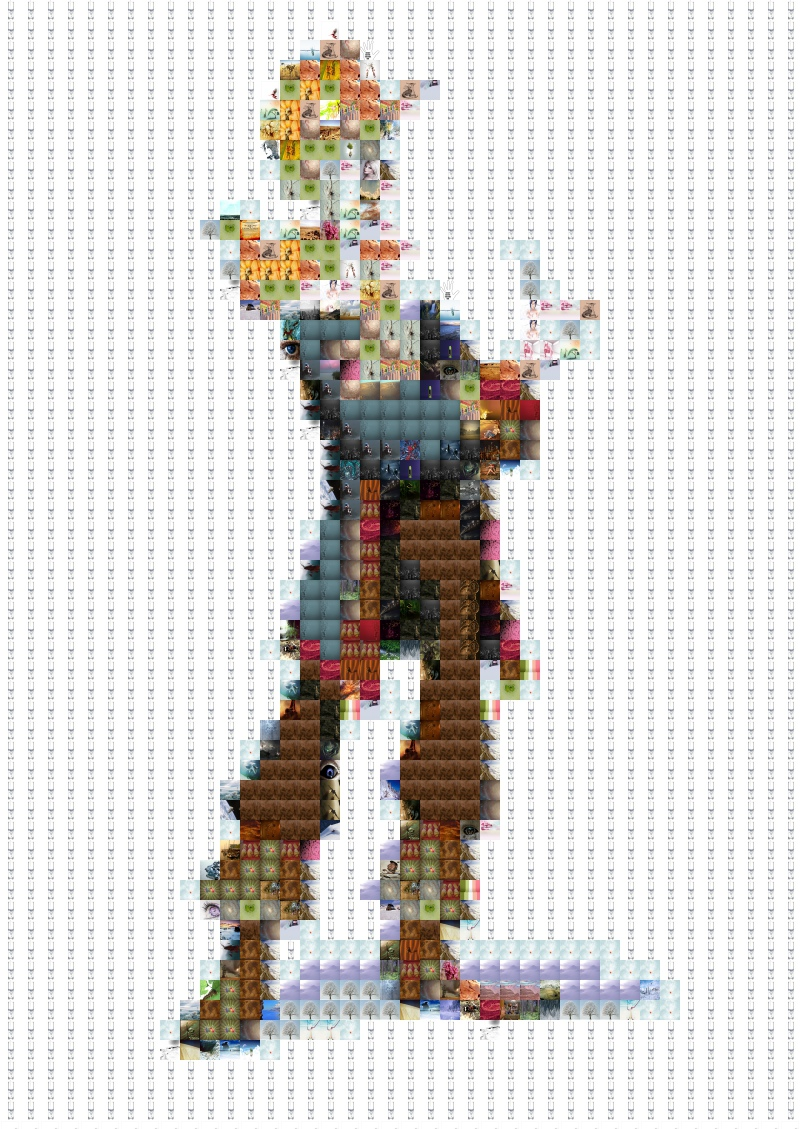
\includegraphics[scale=0.36]{guybrushmse.jpg}
\end{figure}
\end{frame}
\begin{frame}
\frametitle{\bf Resultat avec Mean Color}
\begin{figure}[H]
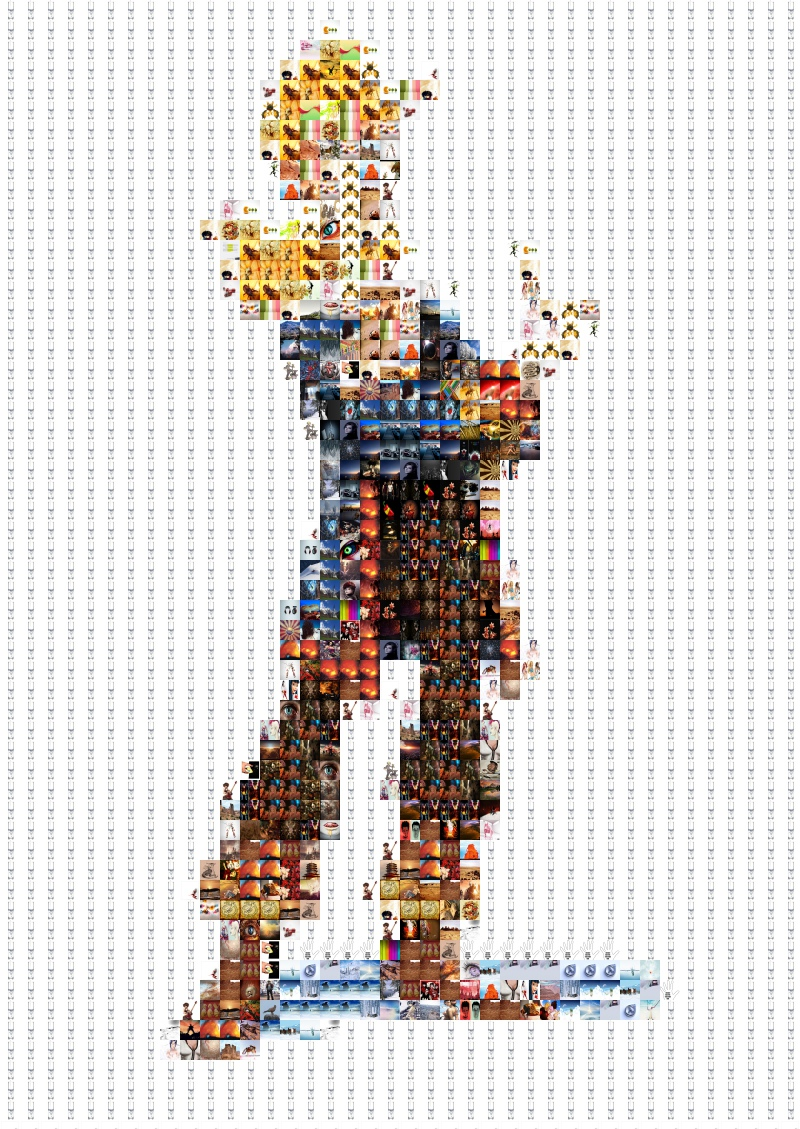
\includegraphics[scale=0.36]{guybrushmeancolor.jpg}
\end{figure}
\end{frame}
\begin{frame}
\frametitle{\bf Resultat avec MCMSE}
\begin{figure}[H]
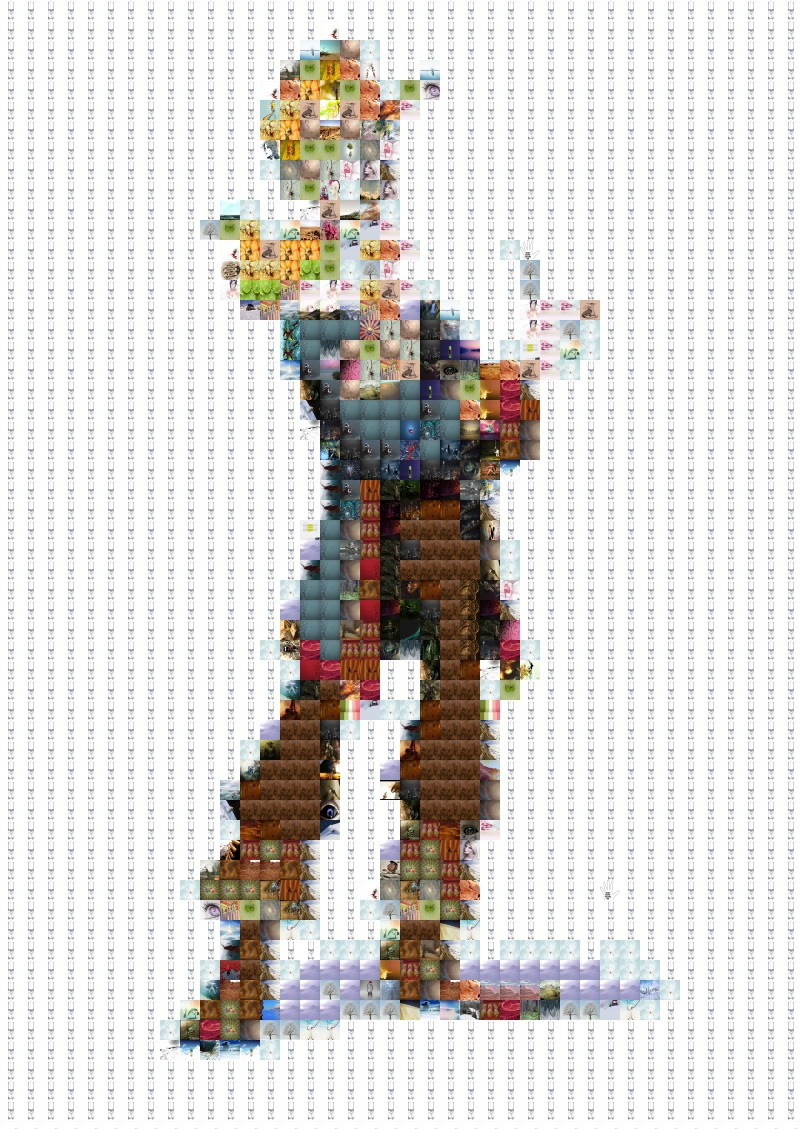
\includegraphics[scale=0.36]{guybrushmcmse.jpg}
\end{figure}
\end{frame}

\begin{frame}
\frametitle{\bf La fin}
Merci pour l'attention!
\end{frame}
%\bibliography{risk}
%\bibliographystyle{chicago}
\end{document}
